\setcounter{section}{0}
\section{Généralités}

Au cours d’un projet de grande ampleur et de longue durée, nombre de facteurs externes et internes peuvent impacter le déroulement de celui-ci. Afin de limiter ces impacts, il est nécessaire de mettre en place une gestion des risques, qui devra permettre d’anticiper les situations à effet négatif sur le déroulement du projet. Pour cela, une démarche en quatre temps est mise en place, consistant à identifier dans un premier temps le risque. L’analyse de ce dernier est alors effectuée, afin de le classifier, estimer sa fréquence d’occurrence et estimer ses impacts. Cela permet par la suite de prévoir des plans de réponse en conséquence, qui pourront être appliqués lorsque la situation à risque surviendra. Enfin, la quatrième étape de suivi permet de contrôler de façon régulière la possible apparition du risque, en réalisant notamment des contrôles et des rapports de façon régulière. \\

\begin{figure}[H]
    \centering
    \label{fig-risque}
    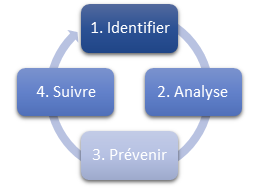
\includegraphics[scale=0.6]{figures/processus_risques.png}
    \caption{Processus de maîtrise des risques}
\end{figure}

Afin d’identifier les risques, il est nécessaire de déterminer dans un premier temps les différents facteurs qui peuvent les déclencher. Il faut cependant distinguer les facteurs humains des facteurs liés au projet, ces derniers étant spécifiques. \\

\section{Facteurs liés à l'humain}

En effet, d’un point de vue humain, la motivation de l’équipe est un facteur très important et ne doit pas être négligé, afin de conserver une productivité favorable. Au regard de la durée du projet, les diminutions de moral peuvent être jugées comme fort probables, et le chef de projet devra y remédier en discutant des problèmes avec son équipe. Afin de surveiller ce risque, un court entretien hebdomadaire personnalisé sera mis en place, au cours duquel les collaborateurs seront invités à noter leur humeur sur une échelle de 0 à 5 et à faire part de leurs remarques sur le déroulement du projet si besoin est. \\
 
Ce projet, de longue durée, devra également être conduit sur une période hivernale, qui augmente fortement le risque de maladie et, a fortiori, de baisse de productivité. Une répartition des tâches modulable est donc à prévoir, afin de permettre un transfert temporaire de productivité. \\
 
\section{Facteurs liés au projet}
 
Concernant les facteurs de risque liés au projet, les livrables devront être terminés dans les temps, afin de ne pas entraîner de glissement dans le planning et impacter d’autres collaborateurs du projet. Les risques de dépassement de délai, entraînant également un dépassement de budget, doivent donc être pris en compte. Afin de prévenir cette situation, les collaborateurs devront utiliser les moyens de communication mis à leur disposition pour signaler toute probabilité de dépassement lié à leurs activités. Ce signalement permettra de mettre en place le plan d’action permettant d’adapter le planning, notamment en réaffectant des collaborateurs en fonction de leur charge de travail. \\
 
Nous pouvons également noter un risque de dépassement des limites du projet, ce dernier étant dans un contexte pouvant porter à confusion, au regard du degré d’intégration de celui-ci. En effet, étant donné la complexité du projet, nombre d’interactions entre les différents acteurs sont à noter. Une étroite collaboration entre le responsable qualité et les autres collaborateurs est donc à prévoir, afin de surveiller la possible émergence de ces facteurs de risque. Le responsable qualité devra ainsi s’assurer que les travaux produits se limitent bien à l’apport de réponses concrètes et cohérentes aux besoins et aux demandes du client. \\

Enfin, l’estimation des temps nécessaires à la réalisation des tâches présente également un risque lié au projet. En effet, si cette étape n’est pas effectuée correctement, les risques de glissement présenteront une fréquence d’occurrence critique. Le manque d’expérience des collaborateurs concernant l’estimation des tâches à réaliser dans ce projet est un important facteur de risque. Afin de prévenir cette situation, l’estimation des durées nécessaires sera effectuée en se positionnant dans les pires cas. \\
